\documentclass{article}
\usepackage{spconf,amsmath,amssymb,graphicx}
\usepackage{booktabs}
\usepackage{cite}
\usepackage{url}
\usepackage{xcolor}
\graphicspath{{figures/}{./}}

% Values still to be filled in by the authors are marked in red; remove before submission.
\newcommand{\tbd}[1]{\textcolor{red}{#1}}

\title{Multi-Representation Anchored Flow Matching\\
for EEG Spatial Super-Resolution}
\name{Ansh Attre, Aadra Sharma, Abhishek Rathore, Arnav Bhavsar}
\address{
School of Computing and Electrical Engineering, \\
Indian Institute of Technology Mandi}

\begin{document}
\maketitle

\begin{abstract}
The task of EEG spatial super-resolution (SR) is to estimate the signals of
unrecorded electrodes from the recorded ones, enabling a high-resolution
montage from low-density headsets. The paradigm also enables the repair of
failed channels. Traditionally, spherical-spline interpolation is the
standard method for this, and deep generative models have recently been
proposed as an alternative. Considering the graph representation as a
suitable fit for EEG SR, we first evaluate the graph-informed flow
matching (GiFlow) framework for recovering 50\% of the electrodes in
participants unseen during training. However, with its published
hyperparameters, the implementation is substantially less accurate than
the spline on the SEED-IV dataset. We attribute this to the training mask,
the heat-kernel source of the flow and rapid overfitting, and address each.
Central to our approach is an adaptive anchoring mechanism: the flow
starts from a per-electrode mixture of classical estimates with learned
weights, so each electrode relies on the estimator that suits it best.
Since the mechanism only replaces the source, it can be generalized to
other generative frameworks. The resulting model reduces the normalized
mean-squared error (NMSE) considerably and outperforms the spline on every
seed. Two controls qualify this gain: the same network trained without
flow matching performs equally well, and covariance kriging, a linear
predictor that requires no training, performs better when training
participants are weighted by their similarity to the test participant. We
also validate the approach on another dataset, DEAP, that shows the same
pattern, with kriging reducing the NMSE considerably.
\end{abstract}

\begin{keywords}
Electroencephalography, spatial super-resolution, flow matching,
spherical spline, kriging
\end{keywords}

\section{Introduction}
\label{sec:intro}

Improving the spatial resolution of EEG by estimating the signals at
electrode sites that were not recorded from the sites that were, known as
spatial super-resolution (SR), can allow low-density and low-cost headsets
to approximate a full montage, which source localization, connectivity
analysis and trained classifiers usually assume. The same reconstruction
pipelines can also be used to interpolate electrodes that fail during a
recording \cite{bigdely2015prep}.

Spherical-spline interpolation \cite{perrin1989spherical} is the standard
method to estimate signals at missing electrodes. It fits a smooth surface
to the observed potentials on a spherical head model and evaluates it at
the missing sites. It requires no training data, but it uses only
electrode positions and ignores both the participant-specific covariance
between electrodes and the temporal structure of the signal. Learned
models aim to exploit this information. Convolutional networks have been
trained to restore or upsample EEG channels \cite{svantesson2021virtual},
diffusion models have been applied to EEG SR \cite{liu2026srgdiff}, and
graph-informed flow matching (GiFlow) \cite{zhang2026giflow} was recently
proposed for spatiotemporal imputation on sensor graphs.

GiFlow is well suited to this task because its flow
\cite{lipman2023flow} starts from a graph-diffused estimate of the missing
values rather than from noise, so the network only needs to learn a
correction. In this work, we apply GiFlow to EEG SR with half of the
electrodes removed, on the SEED-IV \cite{zheng2019emotionmeter} and DEAP
\cite{koelstra2012deap} datasets, with all evaluation on held-out
participants. Our contributions are:
\begin{itemize}
\setlength{\itemsep}{0pt}
\item \emph{multi-representation anchoring}, an adaptive mechanism that
starts the flow from a learned per-electrode mixture of classical
reconstructions and, together with full-montage training and step-level
early stopping, significantly reduces the NMSE of GiFlow on the SEED-IV
and DEAP datasets;
\item an analysis of why GiFlow underperforms on EEG, including a
regression control strategy (the same network without flow matching) that
isolates the contribution of flow matching;
\item a proposed participant-weighted covariance kriging that matches
(within 1\%) or outperforms all learned models we evaluated on both the SEED-IV (62 electrodes) and the DEAP
(32 electrodes) datasets.
\end{itemize}

The anchoring is adaptive in two respects. The mixture weights are learned
for each electrode, so the source draws on whichever representation (graph
diffusion, spatial smoothness or the empirical covariance) best predicts
that electrode, and estimators can be added without changing the network.
Participant-weighted kriging, in turn, adapts the covariance to each new
participant. Since the mechanism only replaces the source of the
generative model, it is not specific to GiFlow: any framework that
transports an initial estimate to the data can be anchored in the same
way, and we also apply it to a flow with SRGDiff-style residual guidance
\cite{liu2026srgdiff}.

\section{Methodology}
\label{sec:method}

\begin{figure*}[t]
\centering
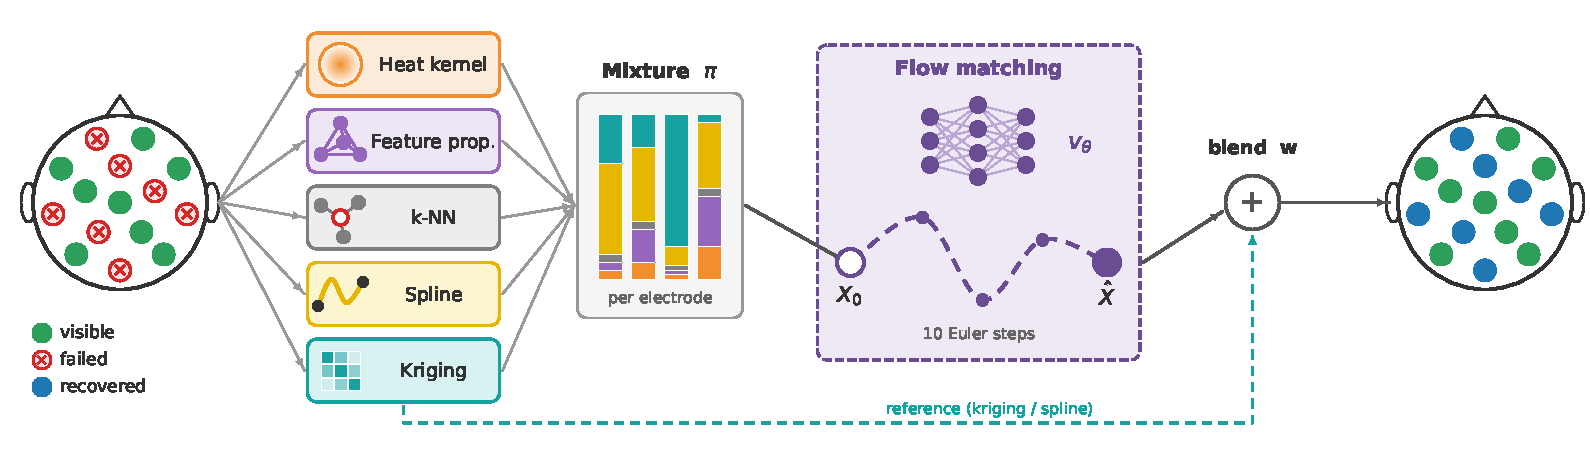
\includegraphics[width=0.9\textwidth]{anchored_flow_pipeline}
\caption{Anchored Flow. Half of the electrodes are missing (red). Up to
five classical estimators reconstruct them, a per-electrode mixture $\pi$
combines the estimates into the source $X_0$, flow matching transports
$X_0$ to $\hat X$ in 10 Euler steps, and the output is blended with the
kriging or spline estimate using a weight $w$ fitted on validation
participants.}
\label{fig:pipeline}
\end{figure*}

\subsection{Problem setting}

A window $X\in\mathbb{R}^{N\times R}$ contains $N$ electrodes ($N=62$ for
the SEED-IV dataset and 32 for the DEAP dataset) and $R$ time samples. For each test participant, a
fixed random half of the electrodes is hidden, simulating missing or
failed electrodes; a different half is drawn for each seed. The model
receives $X_{\mathrm{cond}}=M\odot X$, where the binary mask $M$ removes
the hidden electrodes, and is evaluated only on the hidden entries.
Training participants have complete montages, reflecting a laboratory that
collects full-montage data once and later reconstructs recordings from new
participants.

\subsection{GiFlow}

GiFlow \cite{zhang2026giflow} is a framework proposed for imputing missing
values of spatiotemporal signals measured on sensor graphs. The GiFlow
framework uses two graphs. For the present task, the nodes of the spatial
graph are the $N$ electrodes, and two electrodes are connected when a
Gaussian kernel of their correlation distance $1-|\rho|$, computed from the
pooled recordings, exceeds 0.1. In the temporal graph, the nodes are the $R$
time samples of a window, and each sample is connected to its neighbours
(a chain). With the Laplacians $L_s$ and $L_t$ of these graphs, the
\emph{heat-kernel source}
$X_0=\exp(-\tau_sL_s)\,X_{\mathrm{cond}}\,\exp(-\tau_tL_t)$ diffuses the
observed values to the hidden entries, with diffusion times
$\tau_s,\tau_t$ fitted in advance. A network $v_\theta$ that alternates
spatial and temporal attention with graph message passing is then trained
by flow matching \cite{lipman2023flow} along the linear path
$X_t=(1-t)X_0+tX$, regressing the velocity $X-X_0$ on the hidden entries.
At inference, $v_\theta$ is integrated from $X_0$ in 10 Euler steps, and
the observed entries of the output are reset to their recorded values, so
only the hidden entries are estimated. Since a source closer to the data
reduces the transport cost $\mathbb{E}\|X-X_0\|^2$ of the flow
\cite{zhang2026giflow}, a more accurate source is expected to improve the
result. We use our own implementation of GiFlow in this work.

Applied as it is to EEG SR, this design has three limitations. (i)~The
heat-kernel source only averages correlated neighbours, so with half of
the electrodes missing it is far from the true signal and the transport
cost is high. (ii)~If the evaluation mask is applied to entire recordings,
the hidden electrodes are also hidden in all training windows and never
serve as targets. (iii)~The network overfits the training participants
within a single epoch, so per-epoch validation selects the first
checkpoint.

\subsection{Anchored Flow}

Anchored Flow (Fig.~\ref{fig:pipeline}) addresses limitations (i)--(iii)
with modifications (A)--(C), respectively.

\emph{(A) Multi-representation anchoring.} The heat-kernel source is
replaced by a per-electrode mixture of $K$ classical estimates $\hat X_k$,
\begin{equation}
X_0^{(n)}=\textstyle\sum_k \pi_{nk}\,\hat X_k^{(n)},\qquad
\pi_{n\cdot}=\operatorname{softmax}(\ell_{n\cdot}),
\end{equation}
where $\hat X_k^{(n)}$ is the $k$-th estimate of electrode $n$, $\pi_{nk}$
its mixture weight, and $\ell_{n\cdot}\in\mathbb{R}^K$ learnable logits.
The estimates represent the hidden signal in complementary ways:
(a)~the heat-kernel source, as discussed earlier; (b)~feature propagation
(FP) \cite{rossi2022unreasonable}, which repeatedly averages over
spatial-graph neighbours and resets the observed entries (40 iterations);
(c)~$k$-NN, the mean of the visible spatial-graph neighbours; (d)~the
spherical spline \cite{perrin1989spherical}, computed from 10-05 electrode
positions, with the cerebellar electrodes CB1/CB2 of the SEED-IV dataset
placed at I1/I2; and (e)~optionally, covariance kriging ($K=4$ or 5). The
logits are fitted on training windows by minimizing the transport cost on
hidden entries and then frozen, so each electrode relies on the estimator
that suits it best.

Of the above, we find that kriging is the most accurate estimator
(Table~\ref{tab:main}). Kriging is the best linear predictor of the hidden
electrodes $h$ given the visible electrodes $v$ \cite{cressie1993statistics},
\begin{equation}
\label{eq:kriging}
\hat X_h=\Sigma_{hv}(\Sigma_{vv}+\lambda I)^{-1}X_v,
\end{equation}
where $\Sigma$ is the second-moment matrix of the training participants
and $\lambda$ is $10^{-2}$ times the mean electrode variance. Whereas the
spline imposes a smoothness prior, kriging uses the empirically observed
inter-electrode correlations.

\emph{(B) Full-montage training.} All electrodes are kept visible in
training windows, and randomly selected whole electrodes (each with
probability 0.5) are hidden as targets. Validation and test windows retain
the evaluation mask.

\emph{(C) Step-level early stopping.} We validate every 25--100 steps,
reduce the learning rate to $10^{-4}$, and add weight decay
($5\times10^{-4}$) and dropout (0.3).

Finally, the output may be blended with the spline or kriging estimate as
$w\hat X_{\mathrm{model}}+(1-w)\hat X_{\mathrm{ref}}$, where $w\in[0,1]$
is fitted by least squares on validation participants.

\emph{(D) Regression control.} As an analytical assessment, rather than a
modification, we test whether the improvement is due to flow matching
itself or to the source and the training protocol. The same network,
source and training protocol are used to predict $X-X_0$ in a single step
at $t=0$, and the prediction is added to $X_0$ once at inference.

\subsection{Participant-weighted kriging}

Kriging (Eq.~(\ref{eq:kriging})) predicts each hidden electrode as a linear combination of
the visible ones, with coefficients given by the covariance $\Sigma$
between electrodes; its accuracy therefore depends on how well $\Sigma$
describes the new participant. A single pooled covariance neglects
inter-individual differences in head shape, electrode placement and
anatomy. We therefore weight the training participants by their
similarity to the new one. For a new participant, we compute the
correlation matrix $C_v$ of the visible electrodes and assign each
training participant $p$ the weight
\begin{equation}
\omega_p\propto\exp\!\big(-d_p/(T\,\mathrm{sd}(d))\big),\qquad
d_p=\|C_v-C^{(p)}_v\|_F,
\end{equation}
where $C^{(p)}_v$ uses the same visible electrodes and $\mathrm{sd}(d)$ is
the standard deviation of $d_p$ over $p$. Kriging then uses
$\sum_p\omega_p\Sigma^{(p)}$ in place of the pooled $\Sigma$, with
$\Sigma^{(p)}$ the second-moment matrix of participant $p$.

Only the visible electrodes of the new participant are used, but $C_v$ is
estimated from all of their test windows; the method is therefore
transductive and requires some prior recording from the participant. A
variant fits one covariance per frequency band ($<4$, 4--8, 8--13, 13--30
and $\geq$30~Hz) and sums the band-wise estimates. The temperature $T$ is
selected on validation participants, and the weighted covariance can also
replace the pooled covariance in the anchored source.

\section{Experiments}
\label{sec:experiments}

\textbf{Data.} The SEED-IV dataset \cite{zheng2019emotionmeter} contains 15
participants recorded with 62 channels. We use a preprocessed version
(4~s segments at 250~Hz, normalized and soft-clipped to $\pm5$), which we
band-pass filter to 0.5--75~Hz and resample to 200~Hz.

The DEAP dataset \cite{koelstra2012deap} contains 32 participants with 32 EEG
channels. From the raw BioSemi recordings, we apply an average reference,
band-pass filter to 0.5--75~Hz, resample to 200~Hz and extract 60 evenly
spaced 5~s segments per participant. As amplitudes differ by two orders
of magnitude across participants, each recording is centred per channel,
scaled by one factor (preserving its topography) and soft-clipped with
$5\tanh(x/5)$, as for the SEED-IV dataset.

Both datasets are divided into non-overlapping 100-sample windows (at most
15{,}000 in total, evenly subsampled). Participants 7, 10 and 15 are held out for testing and 6 and 12
for validation; the remainder are used for training. Signals are
standardized using training statistics.

\textbf{Metrics.} NMSE is the squared error summed over all hidden entries,
divided by their total energy. Results are given as mean $\pm$
population standard deviation over seeds 0, 1 and 2. The NMSE definition
is consequential: averaging per window and channel instead emphasizes
low-power channels and at least doubles the spline's NMSE on our data
(0.14 to 0.30 for seed 0).

\textbf{Implementation.} The network has a hidden size of 64 and four
propagation layers, and it is trained with Adam at a batch size of 32,
keeping an exponential moving average of its weights. Experiments on the
SEED-IV dataset were run on Kaggle T4 GPUs and those on the DEAP dataset
on an RTX 4050 GPU. All quantities other than the network weights, namely
the mixture logits, the blend weight and the kriging temperature, are
fitted on training or validation data only.

\section{Results}
\label{sec:results}

\begin{table}[t]
\centering
\small
\caption{NMSE (lower is better) for 50\% electrode loss on held-out
participants, mean $\pm$ SD over 3 seeds. Learned models other than
published GiFlow are blended with their reference estimate. --: not evaluated.}
\label{tab:main}
\setlength{\tabcolsep}{3pt}
\begin{tabular}{@{}lcc@{}}
\toprule
Method & SEED-IV & DEAP\\
\midrule
\multicolumn{3}{@{}l}{\emph{Interpolation (no training)}}\\
$k$-NN & 0.291 $\pm$ 0.007 & 0.946 $\pm$ 0.084\\
Feature propagation & 0.322 $\pm$ 0.008 & 0.829 $\pm$ 0.081\\
Spherical spline & 0.150 $\pm$ 0.006 & 0.981 $\pm$ 0.156\\
Kriging, pooled & 0.127 $\pm$ 0.010 & 0.548 $\pm$ 0.060\\
Kriging, participant-weighted & \textbf{0.116} $\pm$ 0.009 & 0.532 $\pm$ 0.056\\
\quad per frequency band & \textbf{0.114} $\pm$ 0.008 & --\\
\midrule
\multicolumn{3}{@{}l}{\emph{Learned}}\\
GiFlow, published hyperparam. & 0.335 $\pm$ 0.018 & 1.660 $\pm$ 0.975\\
Anchored Flow, spline source & 0.136 $\pm$ 0.007 & 0.677 $\pm$ 0.058\\
Regression control (no flow) & 0.133 $\pm$ 0.008 & 0.623 $\pm$ 0.032\\
Anchored Flow, + kriging & 0.127 $\pm$ 0.010 & 0.543 $\pm$ 0.053\\
\quad participant-weighted & \textbf{0.116} $\pm$ 0.009 & \textbf{0.527} $\pm$ 0.050\\
SRG-style flow, + kriging & 0.127 $\pm$ 0.010 & --\\
\bottomrule
\end{tabular}
\end{table}

\begin{table}[t]
\centering
\small
\caption{Ablation on the SEED-IV dataset, adding one modification at a time to GiFlow
with published hyperparameters (NMSE of the model alone and blended
with FP in the first modified row and with the spline thereafter).}
\label{tab:ablation}
\setlength{\tabcolsep}{4pt}
\begin{tabular}{@{}lcc@{}}
\toprule
Configuration & Model & Blend\\
\midrule
Published hyperparameters & 0.3350 & --\\
+ full montage, mixed source & 0.2381 & 0.2196\\
+ spline in the mixture & 0.1511 & 0.1452\\
+ validate every 100 steps & 0.1507 & 0.1450\\
+ learning rate $10^{-4}$ & 0.1405 & 0.1394\\
+ weight decay, dropout & 0.1367 & 0.1357\\
+ validate every 25 steps & 0.1364 & 0.1346\\
\bottomrule
\end{tabular}
\end{table}

Table~\ref{tab:main} lists the interpolation methods, which require no
training, in its upper half and the learned models in its lower half.

\textbf{(A) SEED-IV dataset.} Among the interpolation methods, the
spherical spline (0.150) is far more accurate than $k$-NN and FP, and
kriging is more accurate still: pooled kriging attains 0.127, and
participant weighting reduces this to 0.116. Band-wise covariances give
0.114, although the variant preferred on validation attains 0.120.

The learned models are, in order: GiFlow with its published
hyperparameters; Anchored Flow with estimators (a)--(d) in the source
(spline source); the regression control (D) with the same source;
Anchored Flow with kriging (e) added to the source, with pooled and with
participant-weighted covariance; and the flow with SRGDiff-style residual
guidance \cite{liu2026srgdiff}, anchored on the same source with pooled
kriging. With its published hyperparameters, GiFlow attains an NMSE of
0.335, more than twice that of the spline and higher than that of $k$-NN.
When the source mixture is learned, the heat kernel receives at most 11\%
of the weight. Anchoring the source, together with modifications (B) and
(C), reduces the NMSE to 0.136, below the spline. The regression control
achieves 0.133 blended and 0.137 alone, matching the flow, so flow
matching itself adds no measurable gain. When kriging is included in the
source, it receives 99\% of the mixture weight, and the flow performs no
better than kriging alone (0.127 vs 0.127, and 0.116 vs 0.116 with
participant weighting). Accordingly, the blend weight $w$ fitted on
validation participants is 0, 0 and 0.30 for the three seeds, i.e., the
blended output is mostly the kriging estimate itself, as the network
learns no correction that generalizes to new participants. The
SRGDiff-style flow on the same source attains the same NMSE (0.127), so
the anchoring transfers to another flow formulation unchanged.

\textbf{Effect of the modifications.} Table~\ref{tab:ablation} reports the
modifications cumulatively. Full-montage training with a mixed source
(heat kernel, FP and $k$-NN) reduces NMSE by 29\%, and including the spline in the mixture, where it
receives 54--56\% of the weight, yields a further 37\% reduction.
Step-level validation alone has no effect, but combined with a lower
learning rate and regularization it moves the best checkpoint to 25--125
steps, and the model alone then outperforms the spline on all three seeds.
The spline-anchored flow in Table~\ref{tab:main} uses the weight-decay
configuration (0.1357).

\textbf{Kriging.} Overall, participant-weighted kriging, which involves no
network training, is more accurate than every learned model without
kriging in its source, and the learned models with kriging in the source
only match it.

\textbf{(B) DEAP dataset.} On the sparser 32-electrode montage, the spline performs
close to the trivial zero predictor (0.981), whereas kriging
reaches 0.548, and 0.532 with participant weighting. GiFlow
with published hyperparameters again underperforms the spline and is
unstable across seeds (0.980, 0.961 and 3.04). The spline-anchored flow
improves on the spline by 31\%, but validation selected the initial or
step-100 weights in all three seeds, so the gain is attributable mainly
to the source mixture (spline 39--43\%, FP 32--33\%, heat kernel
21--24\%). The regression control, which continued to improve for longer,
performs better (0.623). With kriging in the source, the flow remains
within 1\% of kriging alone (0.527 vs 0.532).

\section{Discussion}
\label{sec:discussion}

Our results lead to three observations. First, protocol choices affected
GiFlow more than any architectural change: a training mask that hid the
evaluated electrodes and per-epoch early stopping each cost more than any
model modification we tested. Second, the source matters more than the
generative model, as the anchored source accounts for most of the
improvement and a network without flow matching performs equally well.
Because anchoring only replaces the source, it applies equally to other
generative frameworks, as the SRGDiff-style flow shows. Third, the
spherical spline is an insufficient reference: a kriging
predictor based on training covariances, weighted towards participants
similar to the new one, matched or outperformed every learned model on
both datasets.
Future work would evaluate settings in which flow models may still be
advantageous, such as contiguous missing regions, very sparse montages and
generative uses such as uncertainty estimation, and reproduce
published diffusion models under the same protocol.

\section{Conclusion}
\label{sec:conclusion}

Anchoring GiFlow to an adaptive mixture of classical estimates, training on
the full montage and applying step-level early stopping reduced its error
by 59\% on the SEED-IV dataset and allowed it to outperform the spherical
spline on unseen participants. The anchoring mechanism is independent of
the network and can be generalized to other generative frameworks.
However, an equivalent network without flow matching performs equally
well, and participant-weighted kriging performs better on both the SEED-IV
and DEAP datasets. We recommend that studies of learned EEG SR report such
linear baselines under a common error definition.

\section{Compliance with ethical standards}
\label{sec:ethics}

This study used only public datasets \cite{zheng2019emotionmeter,koelstra2012deap};
ethical approval was not required.

\section{Acknowledgments}
\label{sec:acknowledgments}


\begin{thebibliography}{9}

\bibitem{bigdely2015prep}
N.~Bigdely-Shamlo et~al.,
``The PREP pipeline: standardized preprocessing for large-scale EEG
analysis,'' \emph{Front. Neuroinform.}, vol.~9, p.~16, 2015.

\bibitem{perrin1989spherical}
F.~Perrin et~al.,
``Spherical splines for scalp potential and current density mapping,''
\emph{Electroencephalogr. Clin. Neurophysiol.}, vol.~72, no.~2,
pp.~184--187, 1989.

\bibitem{svantesson2021virtual}
M.~Svantesson et~al.,
``Virtual EEG-electrodes: Convolutional neural networks as a method for
upsampling or restoring channels,'' \emph{J. Neurosci. Methods},
vol.~355, p.~109126, 2021.

\bibitem{liu2026srgdiff}
H.~Liu, L.~Zhou, Z.~Yang, and C.~Yao,
``Step-aware residual-guided diffusion for EEG spatial super-resolution,''
in \emph{Proc. ICLR}, 2026.

\bibitem{zhang2026giflow}
Z.~Zhang, A.~Einizade, J.~H. Giraldo, and O.~Fink,
``Spatiotemporal imputation with graph-informed flow matching,''
arXiv:2606.06682, 2026.

\bibitem{lipman2023flow}
Y.~Lipman et~al.,
``Flow matching for generative modeling,''
in \emph{Proc. ICLR}, 2023.

\bibitem{zheng2019emotionmeter}
W.-L. Zheng et~al.,
``EmotionMeter: A multimodal framework for recognizing human emotions,''
\emph{IEEE Trans. Cybern.}, vol.~49, no.~3, pp.~1110--1122, 2019.

\bibitem{koelstra2012deap}
S.~Koelstra et~al.,
``DEAP: A database for emotion analysis using physiological signals,''
\emph{IEEE Trans. Affect. Comput.}, vol.~3, no.~1, pp.~18--31, 2012.

\bibitem{rossi2022unreasonable}
E.~Rossi et~al.,
``On the unreasonable effectiveness of feature propagation in learning on
graphs with missing node features,''
in \emph{Proc. LoG}, 2022.

\bibitem{cressie1993statistics}
N.~A.~C. Cressie, \emph{Statistics for Spatial Data}, Wiley, 1993.

\end{thebibliography}
\end{document}
